\documentclass[11pt, oneside]{article}   	% use "amsart" instead of "article" for AMSLaTeX format
\usepackage{geometry}                		% See geometry.pdf to learn the layout options. There are lots.
\geometry{letterpaper}                   		% ... or a4paper or a5paper or ... 
%\geometry{landscape}                		% Activate for rotated page geometry
%\usepackage[parfill]{parskip}    		% Activate to begin paragraphs with an empty line rather than an indent
\usepackage{graphicx}				% Use pdf, png, jpg, or eps§ with pdflatex; use eps in DVI mode
								% TeX will automatically convert eps --> pdf in pdflatex		
\usepackage{amssymb}

%SetFonts

%SetFonts


\title{ME 459 Assignment 6}
\author{Jackson Fox}
\date{Due 10/28/2021}							% Activate to display a given date or no date

\begin{document}
\maketitle
\section*{Problem 3}
\subsection*{a)}
A merge conflict occurs when there is a difference in two items being merged together, usually this is the combination of two branches.  If I am committing a branch of code that I have been working on back to the main branch, and git finds a piece of data that I changed that has already been modified in the main branch compared to when I created the branch from main, then a merge conflict occurs as my branch cannot be committed without completely overwriting whatever other changes have occurred to the data in question since my branch creation.
\subsection*{b)}
	\subsection*{i.)} Something.c has three main output sections, each containing conflicts between the feature and main branches. The program starts with printing "Hello world!" with the w lowercase in the main and a lower and capital version in the feature.  The program then lists either the numbers 2-9 on a line in main or 0 - 8, repeating each number from 1-7, in the feature.  The program then returns either an accumulation value about the amount of even numbers from 1 to 7 in main or the value of 7!, both calculated using for loops.
	\subsection*{ii.)}
	Though there was no conflict on the hello world lines, the instructions said to keep the line from main, which included the lower case "world", so I deleted the upper case line from the feature version being merged in.
	\newline
The remaining differences I reconciled using the built in conflict resolver in VS Code.  I was able to select if I wanted to include the main, feature or both versions of the changes in the final file, which I selected based on the instructions.  See below for screenshot.
\newpage
		\begin{figure} [h]
			\centering
			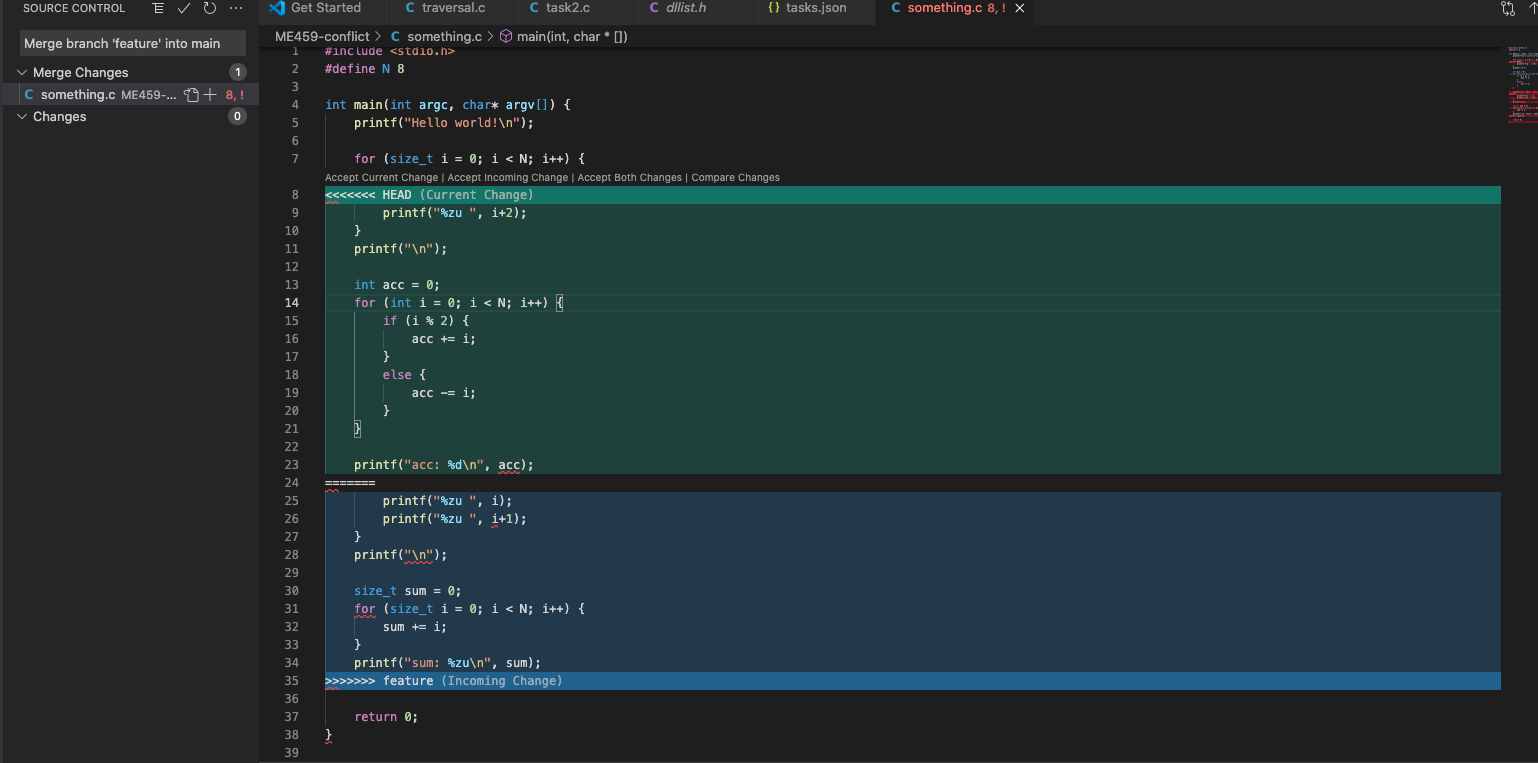
\includegraphics[width=150 mm]{prob3ss.png}
			\caption{VS Code window showing the differences between the feature and main branch versions of the file}
		\end{figure}


After this point, I deleted the main version of the counting method, and then included both changes to get the accumulation and sum portions of the code.  I had to do some slight rearranging to make sure that everything was properly ordered in the file when finally saved.  
\section*{Problem 4}
\subsection*{a)}
\subsection*{i.)} \#29
\subsection*{ii.)}Passed
\subsection*{iii.)} 2:59
\subsection*{b)}
\subsection*{i.)} Test
\subsection*{ii.)} Yes
\subsection*{iii.)} It tested task 2 with 4, 8, 16 and 25 with the inputs from the command line
\subsection*{iv.)} 1 second
\newline
\newline
Using CI enables you to see quickly if changes that have been committed will build and/or test successfully, without requiring you to pull a full copy of the newly merged repo and attempt to run the program yourself.  In the context of working with teams, there is the added advantage of knowing immediately after commits which code/who submitted the code that is causing an issue in the build or successful test of the program/project.  This could save lots of time digging through code to understand when an issue arose or whose code caused the problem.
\end{document}  